\section{Project Management}
\label{sec:Management}

\subsection{Team Structure}
\label{sec:Team}

\emph{Faculty Mentor:}\par
\hspace{1cm} \textbf{Andrew Renshaw}\par
\hspace{1cm} Physics Department\par
\hspace{1cm} \url{arenshaw@central.uh.edu}\par
\vspace{.1in}

\emph{Project Leader:}\par
\hspace{1cm} \textbf{Reed Masek}\par
\hspace{1cm} Physics B.S., Spring 2020\par
\hspace{1cm} \url{rbmasek@uh.edu}\par
\vspace{.1in}

\emph{Team Coordinators:}\par
\hspace{1cm} \textbf{Jimish Patel}\par
\hspace{1cm} Physics B.S., Spring 2020\par
\hspace{1cm} \url{jimishpatel75@gmail.com}\par
\vspace{.05in}
\hspace{1cm} \textbf{Michael Butowicz}\par
\hspace{1cm}  Computer Science B.S., Fall 2020\par
\hspace{1cm} \url{mbutowicz@gmail.com}\par
\vspace{.05in}
\hspace{1cm} \textbf{Taylor Hill}\par
\hspace{1cm} Physics B.S., Spring 2019\par
\hspace{1cm} \url{tdhill92@gmail.com}\par

\begin{figure}[!h]
  \begin{center}
    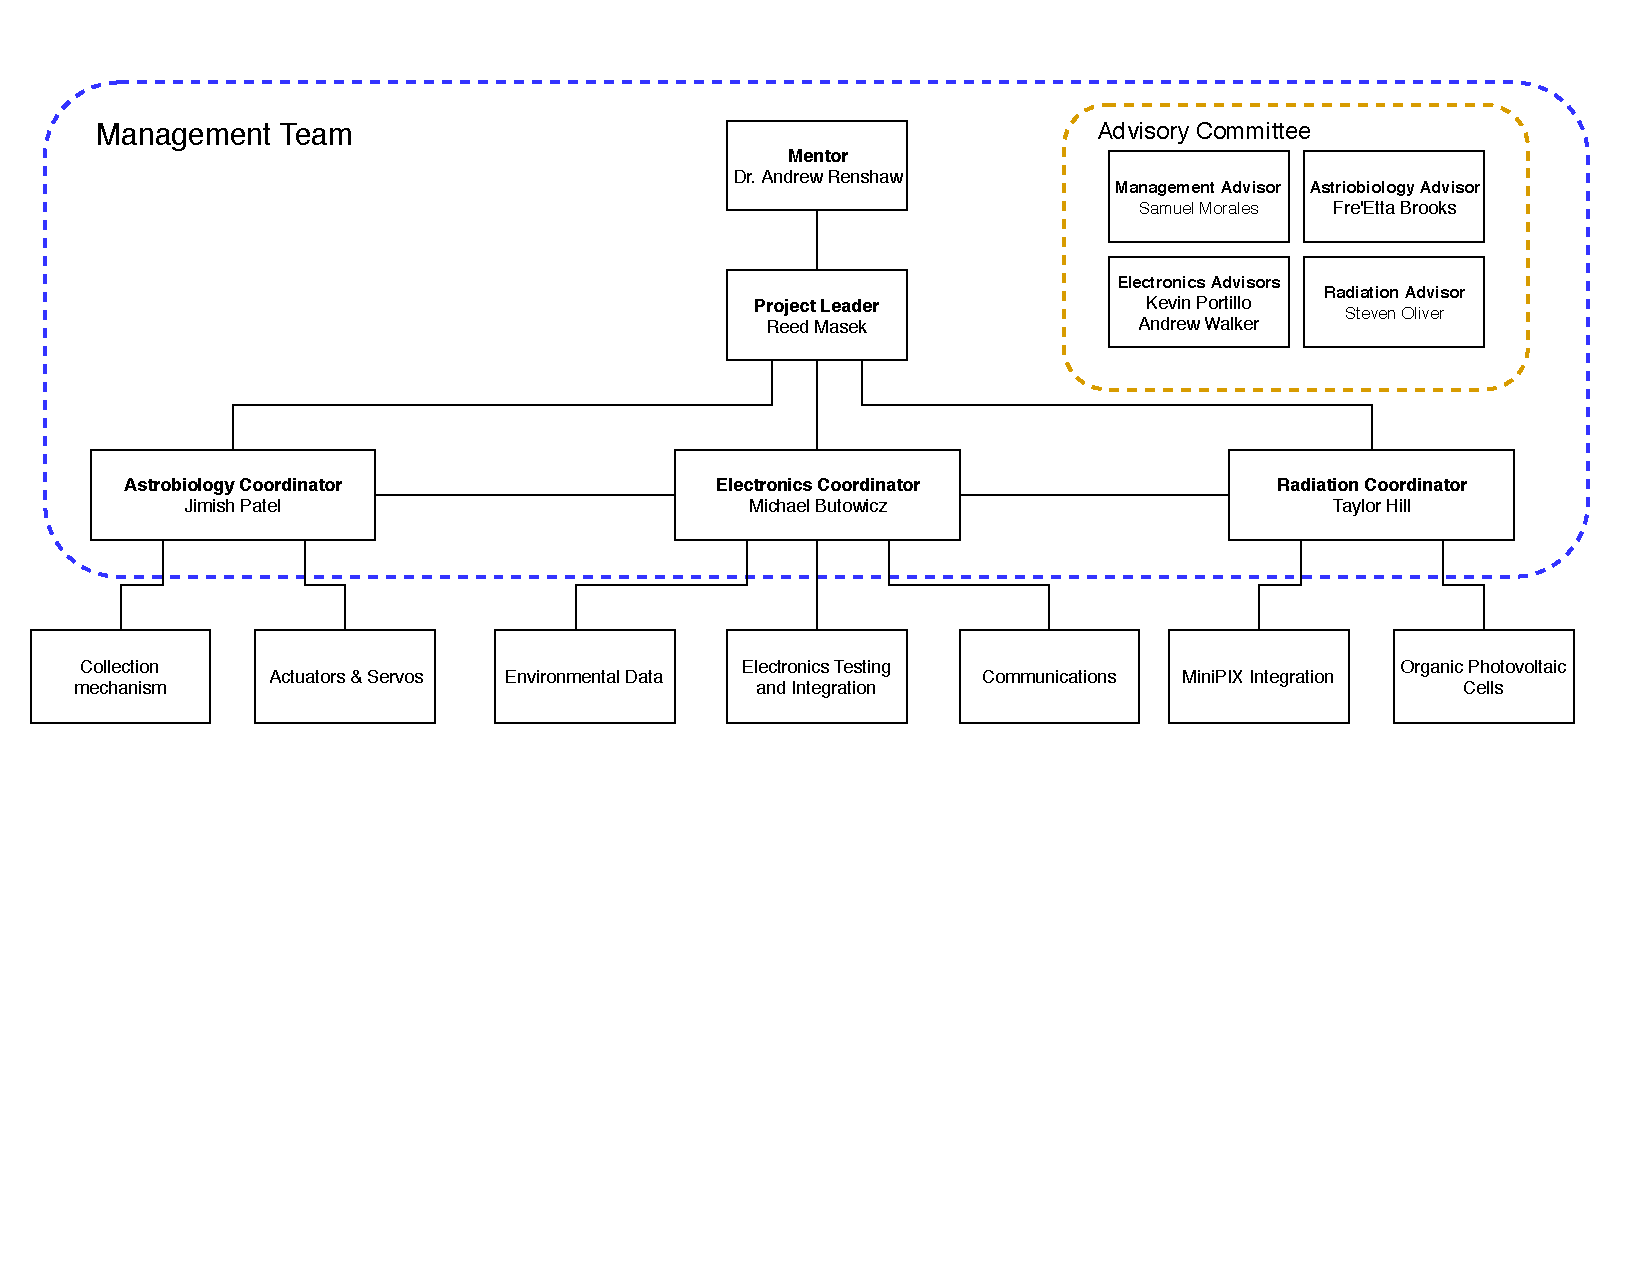
\includegraphics[width=1\textwidth]{./Figures/TeamRoleTree.pdf}
    \caption{Team role tree for the current SORA 2.0 UH team.}
    \label{fig:Roles} 
  \end{center}
\end{figure}

\subsection{Roles and Responsibilities}
\label{sec:Roles}
\begin{itemize}
\item PI – Dr. Andrew Renshaw
	\begin{itemize}
	\item Attend weekly team meetings and provide general research team guidance
	\item Review project design and final products for submission to HASP
	\item Attend monthly teleconferences.
	\item Equipment procurement
	\end{itemize}
\item Project Leader - Reed Masek
	\begin{itemize}
	\item Interface with HASP Flight Control Team and act as team main point of contact
	\item Compile monthly reports and submit to HASP
	\item Attend monthly teleconference with HASP
	\item Coordinate with PI on administration tasks and internal group business
        \item Periodically check-in with team coordinators regarding the team's progress
        \item Coordinate meetings and assign tasks with deadlines
	\item Approve designs, tests, ideas, and any work related to HASP and payload
	\item Final decisions on staffing (staffing decisions will be a group decision overall)
	\end{itemize}
\item Electronics and Communications Coordinator - Michael Butowicz
	\begin{itemize}
	\item Do necessary reserach for finalizing work
	\item Coordinate information, tasks, and deadlines with subgroup
	\item Approve work done by subsystem team
	\item Write bimonthly updates along with detailed reports from subsytem meetings
	\item Make detailed presentations, if necessary, for weekly team meetings
	\item Report to project leader and PI with any project changes, issues encountered, and any external communications.
	\item CC PI and Project Leader in all emails for external communications
	\item Perform other such duties as the Project Leader or PI may specify
	\end{itemize}
\item Astrobiology Coordinator - Jimish Patel
	\begin{itemize}
	\item Do necessary reserach for finalizing work
	\item Coordinate information, tasks, and deadlines with subgroup
	\item Approve work done by subsystem team
	\item Write bimonthly updates along with detailed reports from subsytem meetings
	\item Make detailed presentations, if necessary, for weekly team meetings
	\item Report to project leader and PI with any project changes, issues encountered, and any external communications.
	\item CC PI and Project Leader in all emails for external communications
	\item Perform other such duties as the Project Leader or PI may specify
	\end{itemize}
\item Radiation Coordinator - Taylor Hill
	\begin{itemize}
	\item Do necessary reserach for finalizing work
	\item Coordinate information, tasks, and deadlines with subgroup
	\item Approve work done by subsystem team
	\item Write bimonthly updates along with detailed reports from subsytem meetings
	\item Make detailed presentations, if necessary, for weekly team meetings
	\item Report to project leader and PI with any project changes, issues encountered, and any external communications.
	\item CC PI and Project Leader in all emails for external communications
	\item Perform other such duties as the Project Leader or PI may specify
	\end{itemize}
\item Team Member
	\begin{itemize}
	\item Do necessary reserach for finalizing work
	\item Coordinate with team and subsystem coordinator
	\item Make detailed presentations, if necessary, for weekly team meetings
	\item Report to project leader and PI with any project changes, issues encountered, and any external communications.
	\item CC PI and Project Leader in all emails for external communications
	\item Perform other such duties as the Project Leader or PI may specify
	\end{itemize}
\end{itemize}


\subsection{Timeline}
\label{sec:Timeline}
\begin{table}[H]
\centering
\caption{Timeline for the 2018 SORA 2.0 Mission}
\label{timeline}
\resizebox{\textwidth}{!}{%
\begin{tabular}{|c|l|}
\hline
\textbf{Month of 2018} & \multicolumn{1}{c|}{\textbf{Description of Work}} \\ \hline
\textbf{January} & \begin{tabular}[c]{@{}l@{}} * Secure funding \\ * Create and finish budget for mission \\ * Make inventory of hardware \\ * Procure hardware/software \\ * Start designs of SORA 2.0 \\ * Update RESU \\ * Upgrade vacuum chamber \\ * Recruit new members \end{tabular} \\ \hline
\textbf{February} & \begin{tabular}[c]{@{}l@{}}
* Continue with work from January.  Funding must be secured by end of March.\\ * Have finished list of inventory\\ * Finalize upgrades to vacuum chamber\\ * Continue recruitment and finalize by end of month.\\ * Continue design work of SORA 2.0\\ * Finish RESU upgrade\end{tabular} \\ \hline
\textbf{March} & \begin{tabular}[c]{@{}l@{}}Obtain funding by the end of this month.  Finish all tasks from the previous two months and transition into building phase.\\ * Have all hardware/software orders in by the end of the month\\ * Begin PSIP, have draft by end of the month\end{tabular} \\ \hline
\textbf{April} & \begin{tabular}[c]{@{}l@{}}* Order remaining items if needed\\ * Finish PSIP by April 25th\\ * RESU and MiniPIX integration and testing\\ * Upgrade clean room and prepare for astrobiology work\end{tabular} \\ \hline
\textbf{May} & \begin{tabular}[c]{@{}l@{}}* PSIP and FLOP development\\ * Finalize integration of RESU and hardware\\ * Continue working on astrobiology upgrades\end{tabular} \\ \hline
\textbf{June} & \begin{tabular}[c]{@{}l@{}}Final PSIP due June 27th\\ *Finalize astrobiology upgrades and ready for integration\\ * Testing in lab\end{tabular} \\ \hline
\textbf{July} & \begin{tabular}[c]{@{}l@{}}Final FLOP due July 31st\\ * Make changes from testing and continue tests\end{tabular} \\ \hline
\textbf{August} & \begin{tabular}[c]{@{}l@{}}Payload Integration (August 4 - 8)\\ *Have all payload work done and ready for flight\end{tabular} \\ \hline
\textbf{September} & * Launch and recovery TBA \\ \hline
\textbf{October} & Debrief and analyze all data from flight \\ \hline
\textbf{November} & Have final report by end of November \\ \hline
\textbf{December} & Final Report due on the 8th \\ \hline
\end{tabular}%
}
\end{table}


\subsection{Funding}
\label{sec:Funding}


%Funding sources will be local contributions - applying for funding through the Physics Department, the College of Natural Science and Mathematics, The University of Houston Division of Research, and local organizations and companies willing to support this endeavor.  
